\documentclass[tikz,border=6mm]{standalone}
\usepackage{amsmath,amssymb}
\usetikzlibrary{arrows.meta,positioning,calc,fit,backgrounds}
% Minimal shared style library (vendored). Spacing: xs 4mm, sm 8mm, md 12mm, lg 20mm, xl 32mm.
% Line weights (ISO 128 series): light 0.7pt tertiary/dotted, regular 1.0pt borders + data/dashed,
% strong 1.4pt primary flow, emphasis 2.0pt one callout max. Weight = importance, spacing = grouping,
% dash = category. Every box pins BOTH minimum width and text width.
\def\wLight{0.7pt}\def\wRegular{1.0pt}\def\wStrong{1.4pt}\def\wEmph{2.0pt}
\definecolor{cTwin}{HTML}{2F855A}\definecolor{cLearn}{HTML}{2B6CB0}\definecolor{cBiz}{HTML}{B7791F}
\definecolor{cExec}{HTML}{805AD5}\definecolor{cNv}{HTML}{76B900}\definecolor{cInk}{HTML}{222222}
\tikzset{
  arch/.style={font=\sffamily, every node/.style={align=center}},
  box/.style={draw=cInk, line width=\wRegular, rounded corners=3pt, minimum height=1.05cm,
    minimum width=3.1cm, text width=2.7cm, font=\sffamily\small, fill=white},
  note/.style={font=\sffamily\scriptsize, text=black!60},
  twin/.style={box, fill=cTwin!10, draw=cTwin!80!black},
  learn/.style={box, fill=cLearn!10, draw=cLearn!80!black},
  biz/.style={box, fill=cBiz!14, draw=cBiz!80!black},
  exec/.style={box, fill=cExec!10, draw=cExec!80!black},
  base/.style={box, fill=black!6, draw=black!55},
  nv/.style={draw=cNv!80!black, line width=\wRegular, dotted, rounded corners=3pt, fill=cNv!8,
    minimum height=0.7cm, minimum width=7.4cm, text width=7.0cm, font=\sffamily\scriptsize},
  lane/.style={font=\sffamily\bfseries\scriptsize, text=black!55, anchor=east, text width=2.6cm, align=right},
  flow-a/.style={draw=cInk, line width=\wStrong, -{Stealth[length=2.6mm]}},
  flow-b/.style={draw=cLearn!70!black, line width=\wRegular, dashed, -{Stealth[length=2.6mm]}},
  flow-c/.style={draw=black!60, line width=\wLight, dotted, -{Stealth[length=2.2mm]}},
  flow-d/.style={draw=cExec!80!black, line width=\wRegular, dash dot, -{Stealth[length=2.4mm]}},
  eq/.style={font=\sffamily\scriptsize, text=black!55, fill=white, inner sep=1.5pt},
}
% math macros shared with the monograph
\providecommand{\V}{\mathcal{V}}\providecommand{\E}{\mathcal{E}}\providecommand{\Rel}{\mathcal{R}}
\providecommand{\N}{\mathcal{N}}\providecommand{\R}{\mathbb{R}}
\newcommand{\sub}[1]{{\sffamily\scriptsize\color{black!60}#1}}

\begin{document}
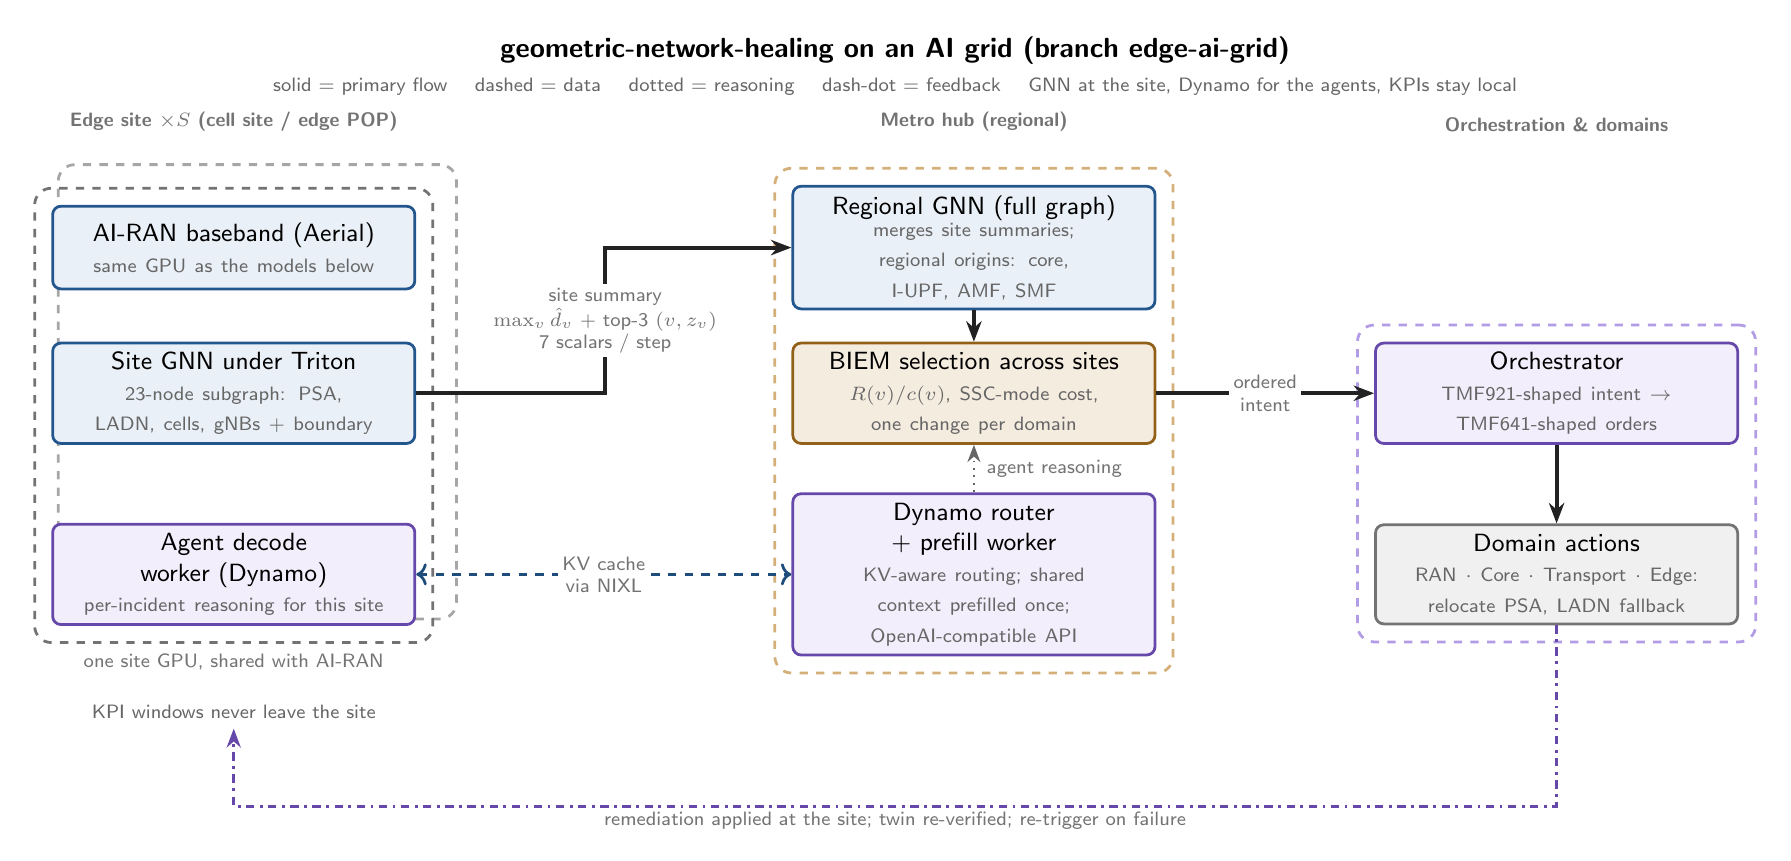
\begin{tikzpicture}[arch, x=1cm, y=1cm]
% Three columns: edge site (x=0), metro hub (x=7.5), orchestration (x=13.5). Row pitch 1.85 (box 1.05 + sm 0.8).
\node[lane, anchor=south, text width=5cm, align=center] at (0, 1.35)    {Edge site $\times S$ (cell site / edge POP)};
\node[lane, anchor=south, text width=5cm, align=center] at (9.4, 1.35)  {Metro hub (regional)};
\node[lane, anchor=south, text width=5cm, align=center] at (16.8, 1.35) {Orchestration \& domains};

% ---- edge site card (one shown, ghost behind suggests S sites)
\node[learn, minimum width=4.6cm, text width=4.2cm] (ran) at (0, 0)     {AI-RAN baseband (Aerial)\\ \sub{same GPU as the models below}};
\node[learn, minimum width=4.6cm, text width=4.2cm] (sgnn) at (0, -1.85) {Site GNN under Triton\\ \sub{23-node subgraph: PSA, LADN, cells, gNBs + boundary}};
\node[exec,  minimum width=4.6cm, text width=4.2cm] (sdec) at (0, -4.15)  {Agent decode worker (Dynamo)\\ \sub{per-incident reasoning for this site}};
\node[note, text width=4.4cm] (kpi) at (0, -5.9) {KPI windows never leave the site};

% ---- metro hub
\node[learn, minimum width=4.6cm, text width=4.2cm] (rgnn) at (9.4, 0)     {Regional GNN (full graph)\\ \sub{merges site summaries;\\ regional origins: core, I-UPF, AMF, SMF}};
\node[biz,   minimum width=4.6cm, text width=4.2cm] (biem) at (9.4, -1.85) {BIEM selection across sites\\ \sub{$R(v)/c(v)$, SSC-mode cost, one change per domain}};
\node[exec,  minimum width=4.6cm, text width=4.2cm] (dyn)  at (9.4, -4.15)  {Dynamo router + prefill worker\\ \sub{KV-aware routing; shared context prefilled once; OpenAI-compatible API}};

% ---- orchestration
\node[exec, minimum width=4.6cm, text width=4.2cm] (orc) at (16.8, -1.85) {Orchestrator\\ \sub{TMF921-shaped intent $\to$ TMF641-shaped orders}};
\node[base, minimum width=4.6cm, text width=4.2cm] (dom) at (16.8, -4.15)  {Domain actions\\ \sub{RAN $\cdot$ Core $\cdot$ Transport $\cdot$ Edge: relocate PSA, LADN fallback}};

% ---- primary flows
\draw[flow-a] (sgnn.east) -- ++(2.4,0) -- ++(0,1.85) node[eq, pos=0.5, align=center] {site summary\\ $\max_v \hat d_v$ + top-3 $(v,z_v)$\\ 7 scalars / step} -- (rgnn.west);
\draw[flow-a] (rgnn) -- (biem);
\draw[flow-a] (biem) -- (orc) node[eq, midway, align=center] {ordered\\ intent};
\draw[flow-a] (orc) -- (dom);
% ---- agents (dotted = reasoning / substrate), KV transfer (dashed = data)
\draw[flow-c] (dyn) -- (biem) node[eq, midway, right, xshift=1mm] {agent reasoning};
\draw[flow-b, <->] (sdec) -- (dyn) node[eq, midway, align=center] {KV cache\\ via NIXL};
% ---- feedback: remediation lands at the site (dash-dot)
\draw[flow-d] (dom.south) -- ++(0,-2.3) -- ++(-16.8,0) node[eq, pos=0.5, below] {remediation applied at the site; twin re-verified; re-trigger on failure} -- (kpi.south);

\begin{scope}[on background layer]
\node[draw=black!35, dashed, rounded corners=6pt, line width=\wRegular, fit=(ran)(sdec), inner sep=6pt, xshift=3mm, yshift=3mm] {};
\node[draw=black!55, dashed, rounded corners=6pt, line width=\wRegular, fit=(ran)(sdec), inner sep=6pt,
      label={[font=\sffamily\scriptsize, text=black!55]below:one site GPU, shared with AI-RAN}] {};
\node[draw=cBiz!60, dashed, rounded corners=6pt, line width=\wRegular, fit=(rgnn)(dyn), inner sep=6pt] {};
\node[draw=cExec!60, dashed, rounded corners=6pt, line width=\wRegular, fit=(orc)(dom), inner sep=6pt] {};
\end{scope}
\node[font=\sffamily\bfseries] at (8.4, 2.5) {geometric-network-healing on an AI grid (branch edge-ai-grid)};
\node[note] at (8.4, 2.05) {solid = primary flow \quad dashed = data \quad dotted = reasoning \quad dash-dot = feedback \quad GNN at the site, Dynamo for the agents, KPIs stay local};
\end{tikzpicture}
\end{document}
